\documentclass[12pt]{beamer}

\usepackage[english]{babel}
\usepackage{graphicx}
\usepackage[utf8]{inputenc}
\usepackage{tikz}

\usetheme{Copenhagen}
\setbeamertemplate{navigation symbols}{}
\setbeamertemplate{bibliography entry title}{}
\setbeamertemplate{bibliography entry location}{}
\setbeamertemplate{bibliography entry note}{}

\usetikzlibrary{shapes}

\title{
  Automated Clustering\\
  of Similar Amendments
}
\author{Jacopo Notarstefano}
\date{June 17, 2016}

\begin{document}
  \begin{frame}[plain]
    \titlepage{}
  \end{frame}

  \begin{frame}{The Problem}
    The Italian Senate is under a Denial of Service attack.

    \vspace{0.5cm}

    A senator in the opposition is using software to generate tons of amendments
    against laws he doesn't want to pass.

    \vspace{0.5cm}

    This software was originally written for \textbf{article spinning}, a black
    hat SEO technique that generates variations of a text using a regex-like
    syntax, sometimes called \textbf{spintax}.
  \end{frame}

  \begin{frame}[fragile]
    \frametitle{An Example of Spintax}

    For example

    \begin{semiverbatim}
\{Hi|Hello\}, this is \{spin syntax|spintax\}.
\end{semiverbatim}

    generates

    \begin{figure}
      \centering
      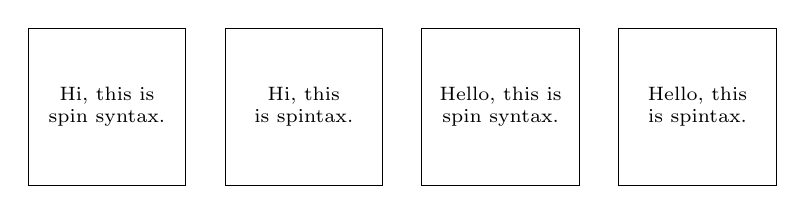
\begin{tikzpicture}
        \draw (   0, 0) rectangle (   2, 2) node[midway,align=center,font=\scriptsize] {Hi, this is\\spin syntax.};
        \draw ( 2.5, 0) rectangle ( 4.5, 2) node[midway,align=center,font=\scriptsize] {Hi, this\\is spintax.};
        \draw (   5, 0) rectangle (   7, 2) node[midway,align=center,font=\scriptsize] {Hello, this is\\spin syntax.};
        \draw ( 7.5, 0) rectangle ( 9.5, 2) node[midway,align=center,font=\scriptsize] {Hello, this\\is spintax.};
      \end{tikzpicture}
    \end{figure}
\end{frame}

  \begin{frame}{The Extent of the Problem}
    \makebox[\textwidth][c]{
      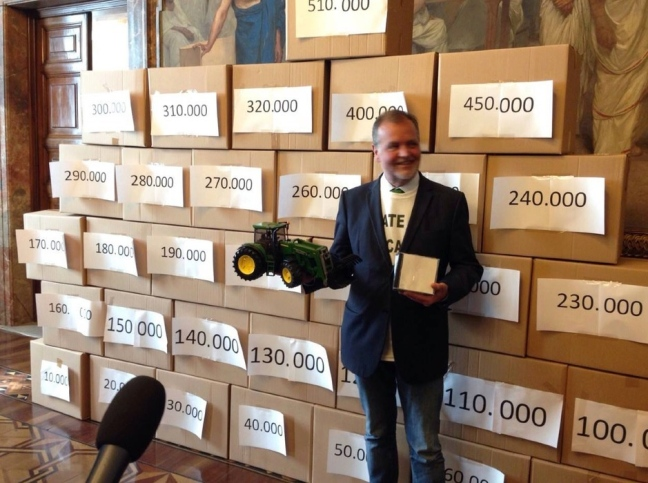
\includegraphics[width=0.9\textwidth]{tex/img/calderoli}
    }
  \end{frame}

  \begin{frame}{Solving the Problem}
    We recognize that the problem we want to solve is an unsupervised clustering
    in an unknown number of clusters.

    \vspace{0.5cm}

    The typical algorithm used to solve this problem is called
    \textbf{Hierarchical Agglomerative Clustering}.
  \end{frame}

  \begin{frame}{HAC in brief, 1/5}
    \begin{figure}
      \centering
      \begin{tikzpicture}
        \node [draw,circle] (A) at (-6, 1) {A};
        \node [draw,circle] (B) at (-4, 2) {B};
        \node [draw,circle] (C) at (-0.5, 2) {C};
        \node [draw,circle] (D) at (0.5, 3) {D};
        \node [draw,circle] (E) at (2, 2) {E};

        \draw[->, -latex] (-7.5, 0.5) -- (2.5, 0.5);
        \draw[->, -latex] (-7, 0) -- (-7, 4.5);

        \path[use as bounding box] (-1,-1) rectangle (10,4);
      \end{tikzpicture}
    \end{figure}
  \end{frame}

  \begin{frame}{HAC in brief, 2/5}
    \begin{figure}
      \centering
      \begin{tikzpicture}
        \node [draw,circle] (A) at (-6, 1) {A};
        \node [draw,circle] (B) at (-4, 2) {B};
        \node [draw,ellipse,rotate=45,minimum width=2cm] (CD) at (0, 2.5) {CD};
        \node [draw,circle] (E) at (2, 2) {E};

        \draw[->, -latex] (-7.5, 0.5) -- (2.5, 0.5);
        \draw[->, -latex] (-7, 0) -- (-7, 4.5);

        \path[use as bounding box] (-1,-1) rectangle (10,4);
      \end{tikzpicture}
    \end{figure}
  \end{frame}

  \begin{frame}{HAC in brief, 3/5}
    \begin{figure}
      \centering
      \begin{tikzpicture}[sloped]
        \node (A) at (-6,0) {A};
        \node (B) at (-4,0) {B};
        \node (C) at (-0.5,0) {C};
        \node (D) at (0.5,0) {D};
        \node (E) at (2,0) {E};

        \node (CD) at (0,1) {};
        \node (CDE) at (1,2) {};

        \draw (C) |- (CD.center);
        \draw (D) |- (CD.center);

        \draw [dashed] (E) |- (CDE.center);
        \draw [dashed] (CD.center) |- (CDE.center);

        \draw [dotted] (-7,1) -- (CD);
        \node [left] (dCD) at (-7,1) {\small \(d(C,D)\)};

        \draw[->,-latex] (-7,0) -- node[above]{distance} (-7,6);
      \end{tikzpicture}
    \end{figure}
  \end{frame}

  \begin{frame}{HAC in brief, 4/5}
    \begin{figure}
      \centering
      \begin{tikzpicture}[sloped]
        \node (A) at (-6,0) {A};
        \node (B) at (-4,0) {B};
        \node (C) at (-0.5,0) {C};
        \node (D) at (0.5,0) {D};
        \node (E) at (2,0) {E};

        \node (AB) at (-4.5,3) {};
        \node (CD) at (0,1) {};
        \node (CDE) at (1,2) {};
        \node (ABCDE) at (-1.5,5) {};

        \draw  (A) |- (AB.center);
        \draw  (B) |- (AB.center);
        \draw  (C) |- (CD.center);
        \draw  (D) |- (CD.center);
        \draw  (E) |- (CDE.center);
        \draw  (CD.center) |- (CDE.center);
        \draw  (AB.center) |- (ABCDE.center);
        \draw  (CDE.center) |- (ABCDE.center);

        \draw[->,-latex] (-7,0) -- node[above]{distance} (-7,6);
      \end{tikzpicture}
    \end{figure}
  \end{frame}

  \begin{frame}{HAC in brief, 5/5}
    \begin{figure}
      \centering
      \begin{tikzpicture}[sloped]
        \node (A) at (-6,0) {A};
        \node (B) at (-4,0) {B};
        \node (C) at (-0.5,0) {C};
        \node (D) at (0.5,0) {D};
        \node (E) at (2,0) {E};

        \node (AB) at (-4.5,3) {};
        \node (CD) at (0,1) {};
        \node (CDE) at (1,2) {};
        \node (ABCDE) at (-1.5,5) {};

        \draw  (A) |- (AB.center);
        \draw  (B) |- (AB.center);
        \draw  (C) |- (CD.center);
        \draw  (D) |- (CD.center);
        \draw  (E) |- (CDE.center);
        \draw  (CD.center) |- (CDE.center);
        \draw  (AB.center) |- (ABCDE.center);
        \draw  (CDE.center) |- (ABCDE.center);

        \draw [thick,red] (-7.5,1.5) -- (2.5,1.5);
        \draw [thick,blue] (-7.5,4.5) -- (2.5,4.5);

        \draw[->,-latex] (-7,0) -- node[above]{distance} (-7,6);
      \end{tikzpicture}
    \end{figure}
  \end{frame}

  \begin{frame}{Jaccard's Distance}
    \begin{definition}[Jaccard's Distance]
      Let \(A\) and \(B\) be two documents, and let \(\text{\texttt{token}}(X)\)
      the function that returns the set of distinct tokens of document \(X\).

      \vspace{0.25cm}

      Then we call \textbf{Jaccard's Distance} the following function:
      \[
        d_{\text{Jaccard}}(A, B) = 1 - \frac
          {\left|\text{\texttt{token}}(A)\cap\text{\texttt{token}}(B)\right|}
          {\left|\text{\texttt{token}}(A)\cup\text{\texttt{token}}(B)\right|}
      \]
    \end{definition}
  \end{frame}

  \begin{frame}{The Final Result}
    \begin{figure}
      \centering
      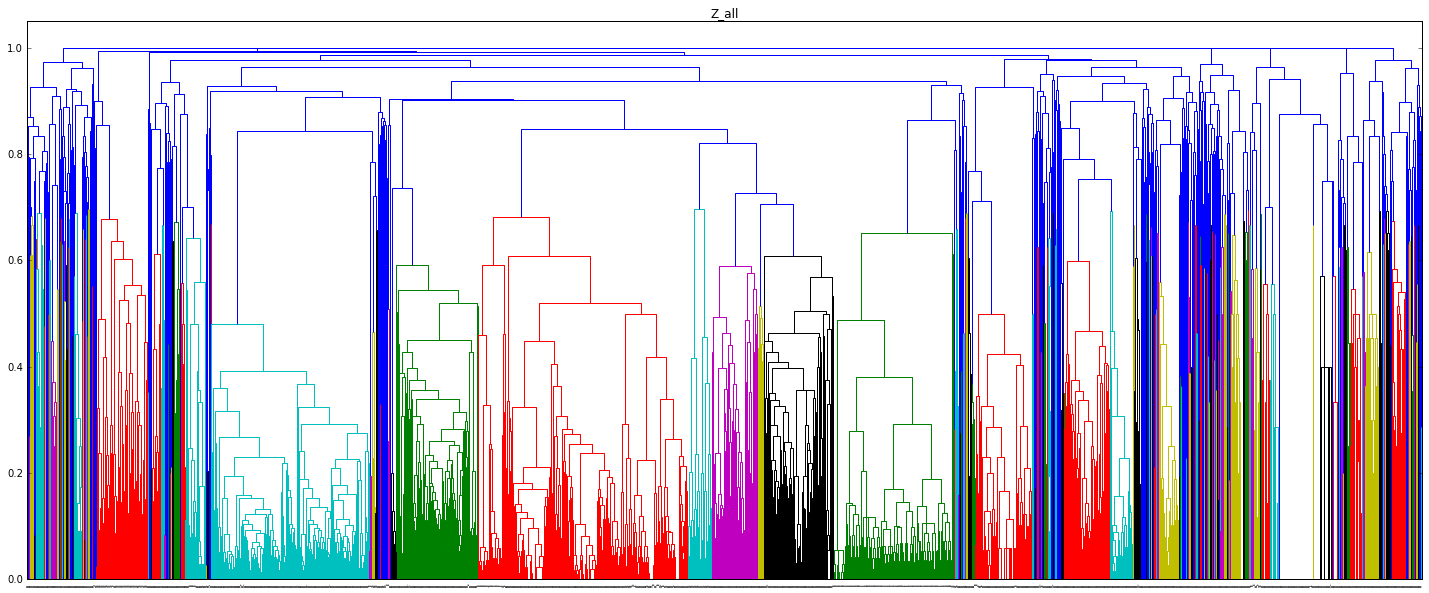
\includegraphics[width=\textwidth]{tex/img/tree-all}
    \end{figure}
  \end{frame}

  \begin{frame}{More Details}
    \makebox[\textwidth][c]{
      \url{https://github.com/jacquerie/senato.py}
    }
  \end{frame}
\end{document}
